\chapter{Arquitectura del sistema}

\section{Diseño general del sistema}

La arquitectura del sistema desarrollado para la plataforma comunitaria de Tejarcillos se basa en el patrón arquitectónico \textbf{Modelo-Vista-Controlador (MVC), lo que permite una separación clara de responsabilidades (Reenskaug, 1979).}, implementado sobre el stack tecnológico \textbf Se utilizó el stack MERN compuesto por MongoDB, Express.js, React y Node.js, tecnologías ampliamente utilizadas para el desarrollo web moderno (MongoDB, Inc., 2025; OpenJS Foundation, 2025a; OpenJS Foundation, 2025b; Meta Platforms, Inc., 2025b). Esta elección arquitectónica permite una separación clara de responsabilidades entre las diferentes capas del sistema, facilitando el mantenimiento, escalabilidad y comprensión del código.

El diseño de la comunicación cliente-servidor se implementó a través de una API RESTful, en línea con los principios planteados por Fielding (2000). La implementación sigue principios de desarrollo modular, donde cada componente tiene responsabilidades específicas y bien definidas.

\subsection*{Arquitectura Backend}
En el backend, la aplicación utiliza \textbf{Express.js con TypeScript} para aprovechar el tipado estático y mejorar la robustez del código. La estructura modular incluye:
\begin{itemize}
  \item \textbf{Controladores}: Gestionan la lógica de negocio y coordinan las operaciones entre modelos y rutas.
  \item \textbf{Modelos}: La persistencia de datos se gestiona mediante {Mongoose}, un ODM para MongoDB que facilita el manejo de esquemas (Automattic, 2025).
  \item \textbf{Rutas}: Definen los endpoints de la API REST y conectan las solicitudes HTTP con los controladores correspondientes.
  \item \textbf{Middlewares}: Proporcionan funcionalidades transversales como autenticación JWT, validación de roles y manejo de archivos.
  \item \textbf{Interfaces}: Definen contratos de datos utilizando TypeScript para garantizar consistencia.
\end{itemize}

\subsection*{Arquitectura Frontend}
El frontend está desarrollado en \textbf{React.js} utilizando componentes funcionales y \textbf{React Router} para la navegación. La estructura modular permite la reutilización de componentes y facilita el mantenimiento:
\begin{itemize}
  \item \textbf{Componentes reutilizables}: Elementos comunes de interfaz.
  \item \textbf{Páginas}: Vistas completas que integran múltiples componentes.
  \item \textbf{Servicios de API}: Centralizan las comunicaciones con el backend.
  \item \textbf{Context API}: Gestión del estado global de autenticación.
\end{itemize}

\subsection*{Comunicación y Seguridad}
La autenticación y autorización se implementó con JSON Web Tokens (JWT), siguiendo el estándar definido por la IETF (Jones, Bradley y Sakimura, 2015). El sistema implementa middleware de seguridad para validar roles de usuario y proteger rutas sensibles.

\subsection*{Mejoras en el Sprint 1}
Durante esta iteración se realizaron mejoras arquitectónicas significativas:
\begin{enumerate}
  \item \textbf{Sistema de categorías}: Se añadió una nueva entidad {Categoria} con su respectivo modelo, controlador y rutas.
  \item \textbf{Optimización del sistema de archivos}: Se mejoró la gestión de imágenes (servidor) y documentos (base de datos).
  \item \textbf{Calendario interactivo}: Integración con endpoints especializados para consultas por rangos de fechas.
  \item \textbf{Mejoras en la persistencia}: Nuevos campos en los modelos ({precio}, {horaEvento}) y referencias a categorías.
\end{enumerate}

\section{Diseño de la persistencia}

La persistencia se diseñó con un \textbf{modelo Entidad-Relación (E-R)} adaptado a MongoDB. Esta decisión permite aprovechar la flexibilidad de una base de datos orientada a documentos manteniendo claridad conceptual.

\subsection*{Modelo Conceptual Actualizado}
Cambios realizados en el Sprint 1:
\begin{itemize}
  \item \textbf{Usuario}: Se mantienen atributos originales ({nombre}, {apellidos}, {email}, {password}, {tipoUsuario}, {codigo}).
  \item {Publicación}: Se añadieron {precio} y {horaEvento}. Se reemplazó el campo {tag} por una referencia a {Categoria}.
  \item {Categoría (nueva)}: Incluye {identificador}, {nombre}, {tipo}. Relación uno a muchos con {Publicación}.
  \item {Comentario}: Sin cambios, mantiene relación con {Usuario} y {Publicación}.
  \item {Archivo y Carpeta}: Relaciones optimizadas y jerarquía mantenida.
\end{itemize}

\begin{figure}[H]
  \centering
    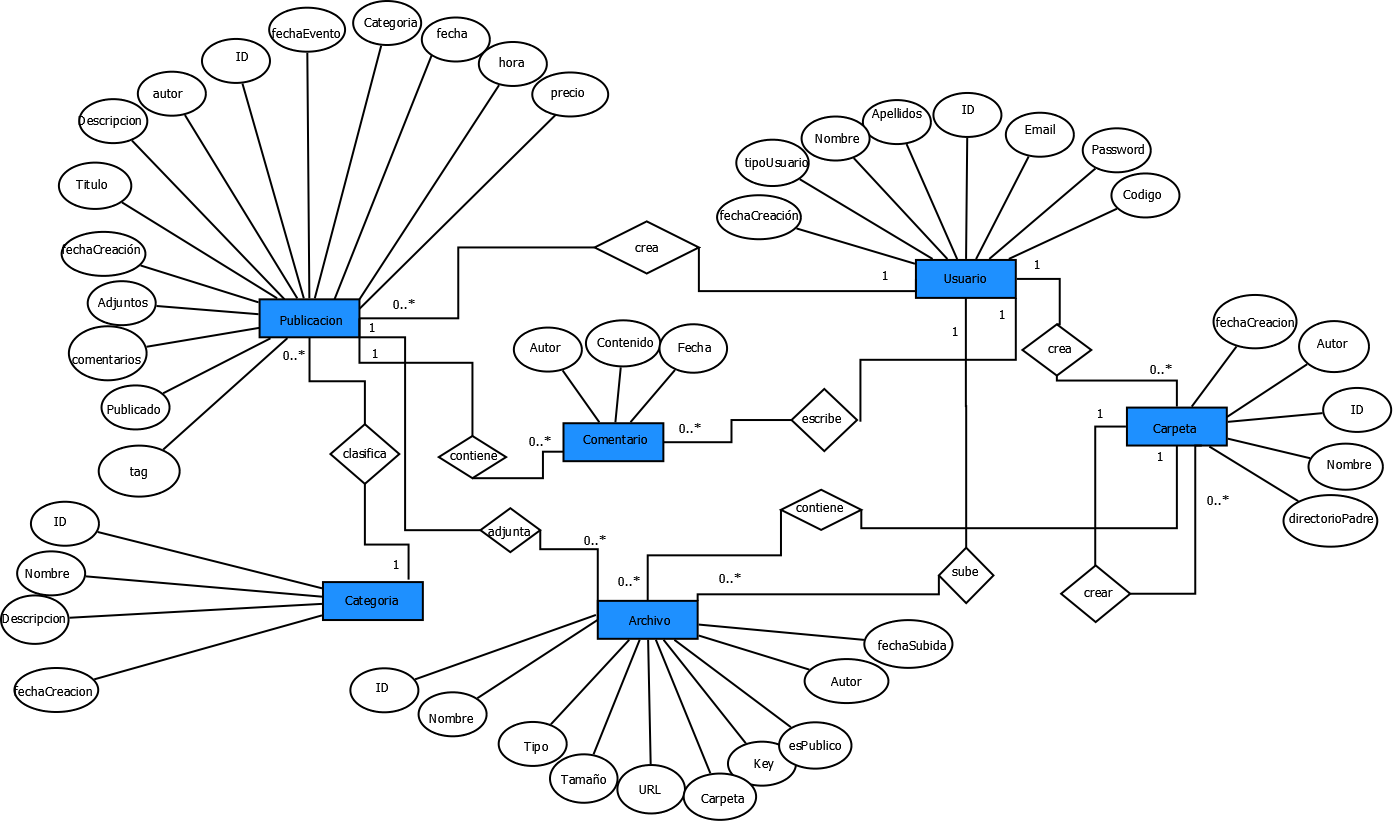
\includegraphics[width=15cm]{project/images/Diagrama1.png}
  \caption{\textbf{Modelo Entidad-Relación del sistema}}
  \label{ERModel}
\end{figure}

\subsection*{Justificación de los cambios}
\begin{enumerate}
  \item Migrar {tag} a entidad {Categoria} mejora integridad y eficiencia en consultas.
  \item Extensión de {Publicacion} permite cubrir emprendimientos y eventos sin nuevas entidades.
  \item Consultas más eficientes gracias a referencias y {populate} de Mongoose.
\end{enumerate}

\subsection*{Estrategia de Almacenamiento de Archivos}
\begin{itemize}
  \item \textbf{Imágenes}: En servidor local (\texttt{/srv/uploads}).
  \item \textbf{Documentos}: En MongoDB mediante GridFS.
\end{itemize}



\section{Diagrama de clases}

El diagrama de clases refleja la arquitectura orientada a objetos, actualizada tras las mejoras del Sprint 1. Incorpora la nueva clase {Categoria} y la extensión de {Publicacion}.

\subsection*{Clases principales}
\begin{itemize}
  \item \textbf{Usuario}: Atributos ({nombre}, {apellidos}, {email}, {password}, {tipoUsuario}, {codigo}). Relaciones: {Publicacion}, {Carpeta}, {Archivo}.
  \item \textbf{Categoria}: Atributos ({identificador}, {nombre}, {tipo}). Relación uno a muchos con {Publicacion}.
  \item \textbf{Publicacion}: Atributos ({titulo}, {contenido}, {fecha}, {adjuntos}, {comentarios}, {publicado}, {precio}, {horaEvento}). Asociación con {Categoria}.
  \item \textbf {Comentario}: Sin cambios, asociado a {Usuario} y {Publicacion}.
  \item \textbf {Archivo y Carpeta}: Mantienen estructura jerárquica y asociación con {Usuario}.
\end{itemize}

\subsection*{Mejoras en el diseño de clases}
\begin{enumerate}
  \item Separación de responsabilidades mediante la clase {Categoria}.
  \item Extensibilidad con nuevos campos en {Publicacion}.
  \item Integridad referencial en relación {Publicacion-Categoria}.
  \item Reutilización de categorías en múltiples publicaciones.
\end{enumerate}

\begin{figure}[H]
  \centering
    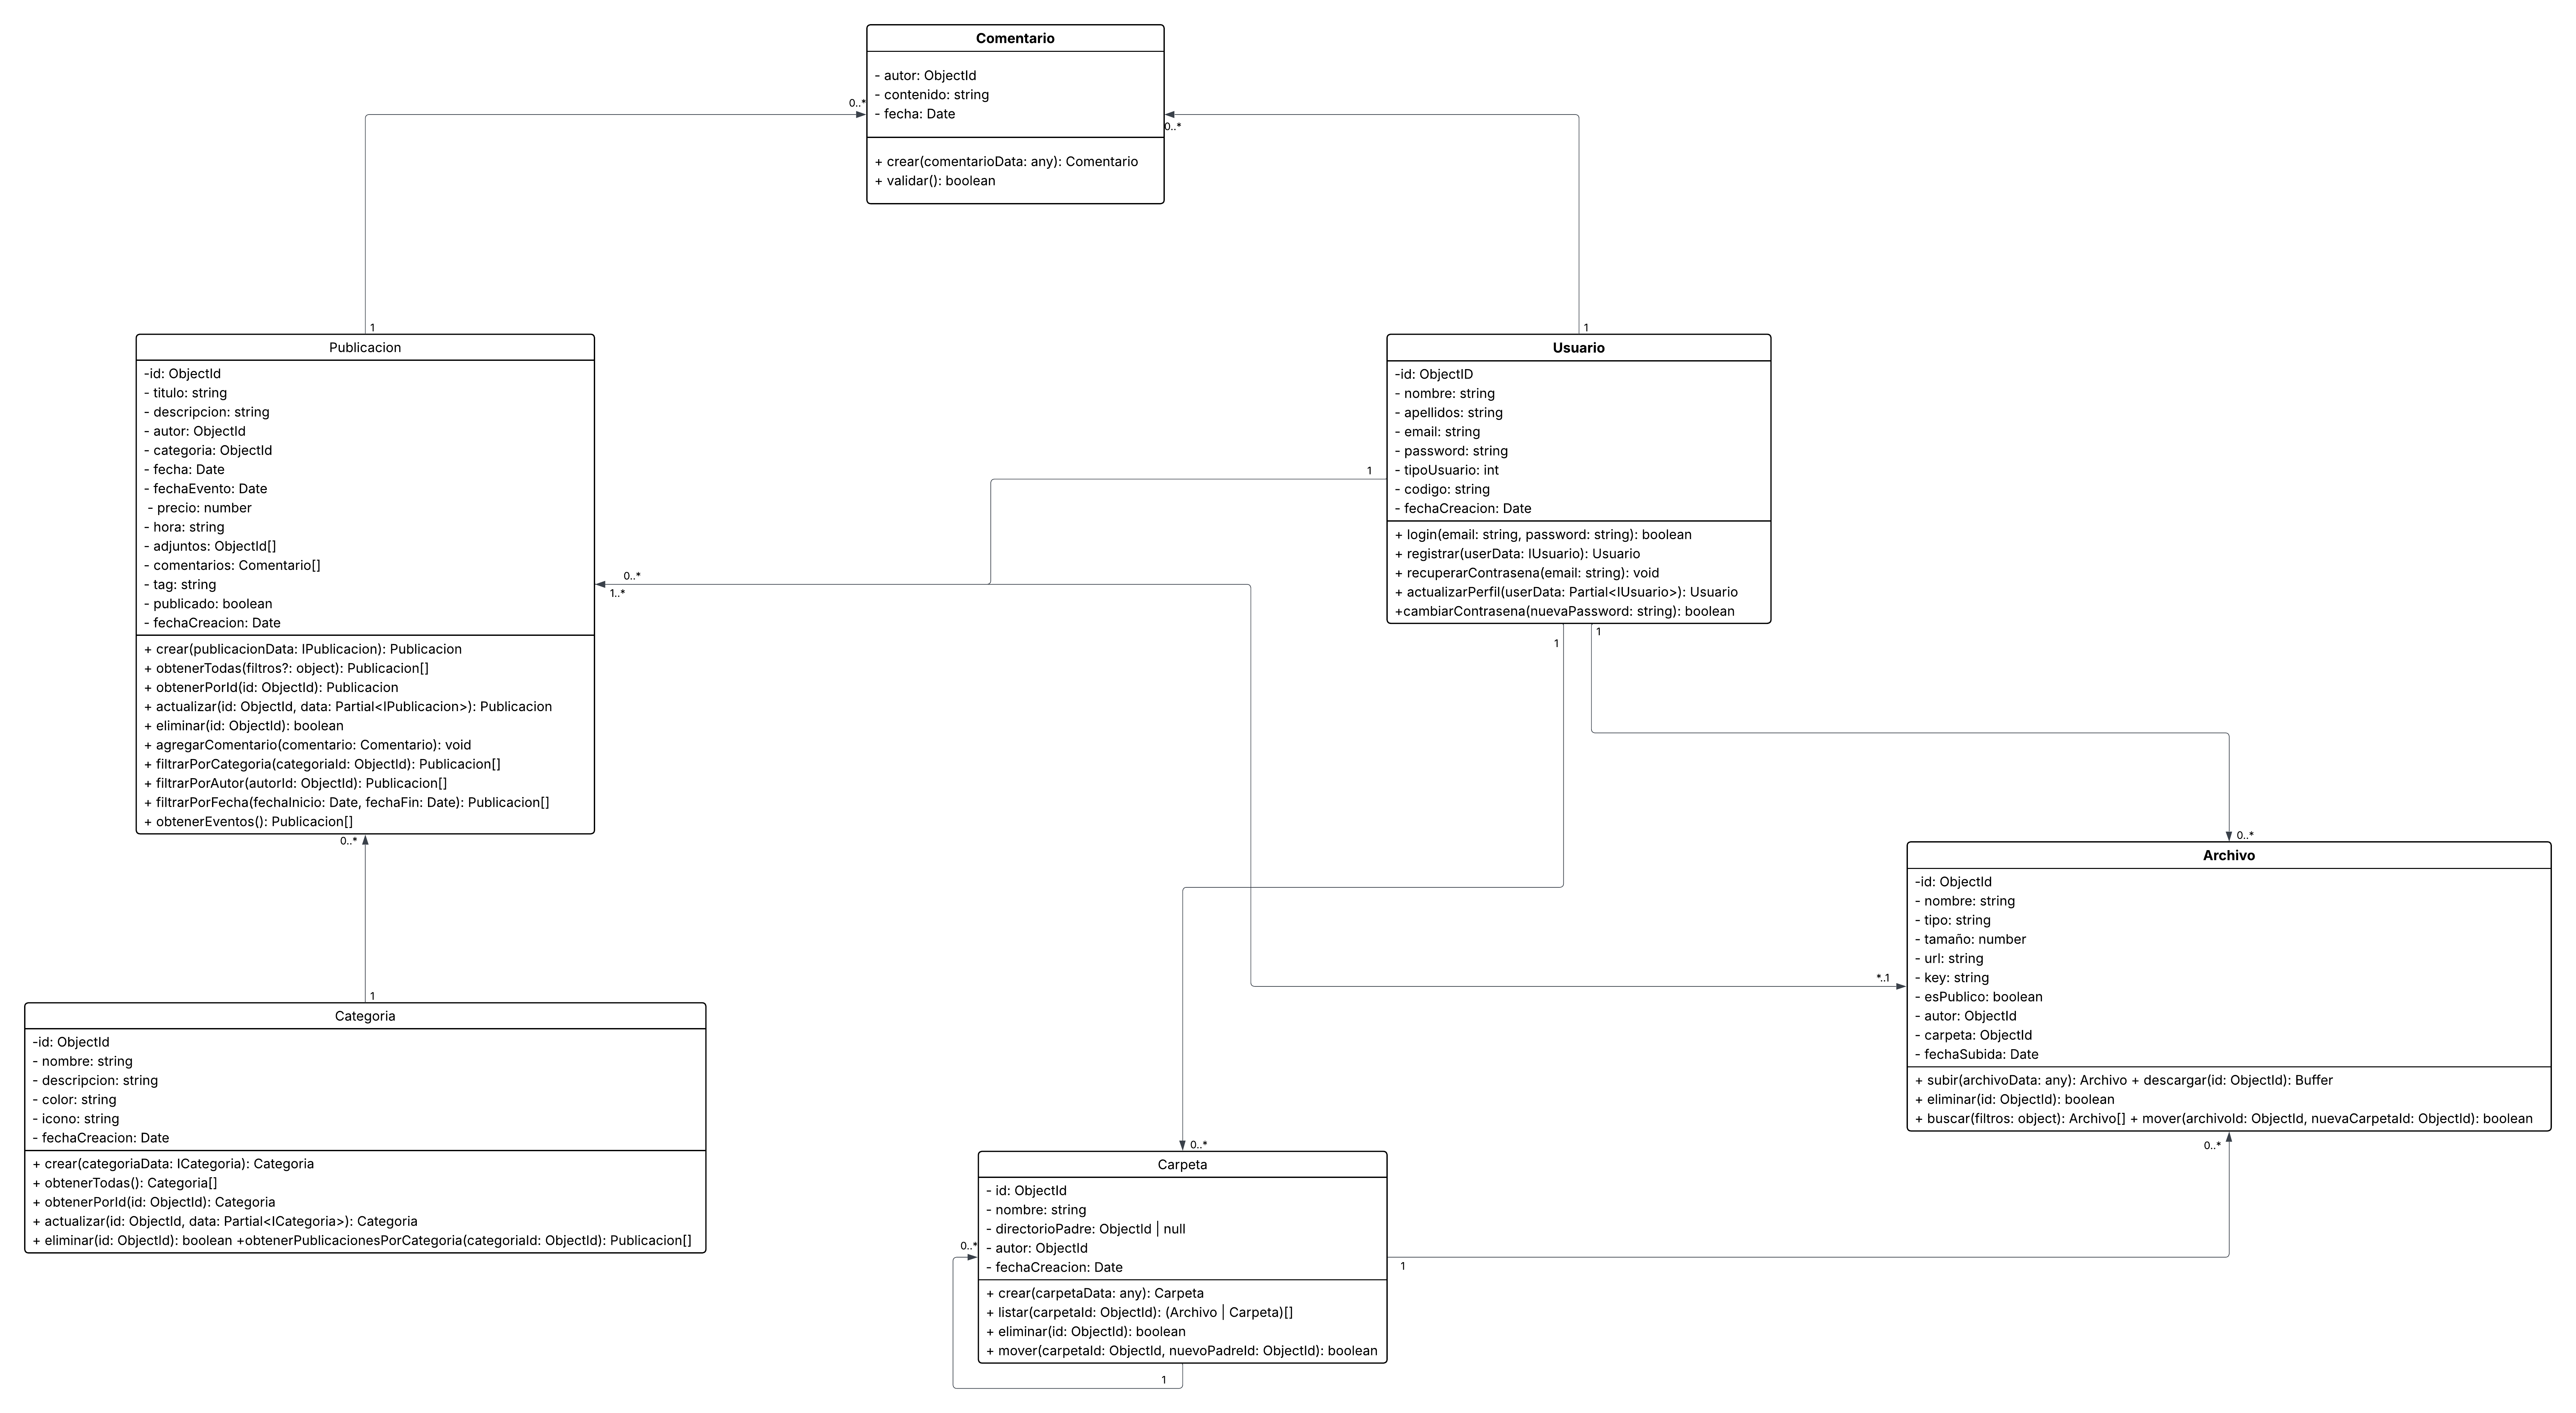
\includegraphics[width=15cm]{project/images/DC.png}
  \caption{\textbf{Diagrama de clases del sistema}}
  \label{DiagramaClases}
\end{figure}



